\documentclass[10pt]{article}
% Shared preamble of the problems/MHD/setup_notes documents.
% Each case document does % Shared preamble of the problems/MHD/setup_notes documents.
% Each case document does % Shared preamble of the problems/MHD/setup_notes documents.
% Each case document does \input{preamble} right after \documentclass.
\usepackage[margin=0.85in]{geometry}
\usepackage[T1]{fontenc}
\usepackage{lmodern}
\usepackage{amsmath,amssymb,bm}
\usepackage{array,booktabs,tabularx,longtable,multirow}
\usepackage{xcolor}
\usepackage{enumitem}
\usepackage[normalem]{ulem}
\usepackage[hyphens]{url}
\usepackage[colorlinks=true,linkcolor=blue!50!black,urlcolor=blue!50!black]{hyperref}
\usepackage{caption}
\usepackage{graphicx}
\setlist{itemsep=1pt,topsep=3pt}
\sloppy
\emergencystretch=3em
\newcolumntype{Y}{>{\raggedright\arraybackslash}X}
\newcolumntype{L}[1]{>{\raggedright\arraybackslash}p{#1}}

% \code{...}: typewriter with breakable underscores (write \_ in the argument).
\makeatletter
\newcommand{\code}[1]{{\def\_{\char`\_\discretionary{}{}{}}\texttt{#1}}}
\makeatother

% --- Common-item marks -------------------------------------------------------
% \cm{x}  solid underline : identical in EVERY case to which the item applies
% \mj{x}  dashed underline: shared by a MAJORITY of those cases, but not all
\newcommand{\cm}[1]{\uline{#1}}
\newcommand{\mj}[1]{\dashuline{#1}}

\newcommand{\commonlegend}{%
\begin{center}
\fcolorbox{black!40}{black!3}{\parbox{0.92\textwidth}{\small
\textbf{How to read the underlines.}
\cm{Solid underline}: the setting (or the code path) is \emph{identical in every case
of \code{problems/MHD} to which it applies} --- all nine cases for general settings, the eight
\code{DSGS\_MHD} cases for DynSGS settings, the three \code{:positivity\_method => "conservative"}
cases for the element limiter.
\mj{Dashed underline}: shared by a \emph{majority} of those cases but not all of them.
No underline: specific to this case or to a minority.
The cross-case comparison is in \code{summary.pdf} of this directory.}}
\end{center}}

% --- Notation ----------------------------------------------------------------
\newcommand{\bq}{\mathbf{q}}
\newcommand{\bv}{\mathbf{v}}
\newcommand{\bmom}{\mathbf{m}}
\newcommand{\bB}{\mathbf{B}}
\newcommand{\bF}{\mathbf{F}}
\newcommand{\Et}{\tilde E}
\newcommand{\eps}{\varepsilon}
\newcommand{\dsgs}{DynSGS}
\newcommand{\CR}{C_R}
\newcommand{\Cmax}{C_{\max}}
\newcommand{\Cmin}{C_{\min}}
\newcommand{\nuc}{\nu_{c}}
\newcommand{\nufl}{\nu_{\mathrm{fl}}}
\newcommand{\commit}{\code{dcc3653}}
\newcommand{\branch}{\code{sm/MHD}}

% Two-column "setting" table: key | value as used | where / remark
\newenvironment{keytable}{%
\par\smallskip\noindent\small
\begin{longtable}{@{}L{0.24\textwidth}L{0.38\textwidth}L{0.32\textwidth}@{}}
\toprule
\textbf{Deck key / item} & \textbf{Value as run} & \textbf{Source / remark}\\
\midrule\endhead
\bottomrule\endfoot}{%
\end{longtable}\par}
 right after \documentclass.
\usepackage[margin=0.85in]{geometry}
\usepackage[T1]{fontenc}
\usepackage{lmodern}
\usepackage{amsmath,amssymb,bm}
\usepackage{array,booktabs,tabularx,longtable,multirow}
\usepackage{xcolor}
\usepackage{enumitem}
\usepackage[normalem]{ulem}
\usepackage[hyphens]{url}
\usepackage[colorlinks=true,linkcolor=blue!50!black,urlcolor=blue!50!black]{hyperref}
\usepackage{caption}
\usepackage{graphicx}
\setlist{itemsep=1pt,topsep=3pt}
\sloppy
\emergencystretch=3em
\newcolumntype{Y}{>{\raggedright\arraybackslash}X}
\newcolumntype{L}[1]{>{\raggedright\arraybackslash}p{#1}}

% \code{...}: typewriter with breakable underscores (write \_ in the argument).
\makeatletter
\newcommand{\code}[1]{{\def\_{\char`\_\discretionary{}{}{}}\texttt{#1}}}
\makeatother

% --- Common-item marks -------------------------------------------------------
% \cm{x}  solid underline : identical in EVERY case to which the item applies
% \mj{x}  dashed underline: shared by a MAJORITY of those cases, but not all
\newcommand{\cm}[1]{\uline{#1}}
\newcommand{\mj}[1]{\dashuline{#1}}

\newcommand{\commonlegend}{%
\begin{center}
\fcolorbox{black!40}{black!3}{\parbox{0.92\textwidth}{\small
\textbf{How to read the underlines.}
\cm{Solid underline}: the setting (or the code path) is \emph{identical in every case
of \code{problems/MHD} to which it applies} --- all nine cases for general settings, the eight
\code{DSGS\_MHD} cases for DynSGS settings, the three \code{:positivity\_method => "conservative"}
cases for the element limiter.
\mj{Dashed underline}: shared by a \emph{majority} of those cases but not all of them.
No underline: specific to this case or to a minority.
The cross-case comparison is in \code{summary.pdf} of this directory.}}
\end{center}}

% --- Notation ----------------------------------------------------------------
\newcommand{\bq}{\mathbf{q}}
\newcommand{\bv}{\mathbf{v}}
\newcommand{\bmom}{\mathbf{m}}
\newcommand{\bB}{\mathbf{B}}
\newcommand{\bF}{\mathbf{F}}
\newcommand{\Et}{\tilde E}
\newcommand{\eps}{\varepsilon}
\newcommand{\dsgs}{DynSGS}
\newcommand{\CR}{C_R}
\newcommand{\Cmax}{C_{\max}}
\newcommand{\Cmin}{C_{\min}}
\newcommand{\nuc}{\nu_{c}}
\newcommand{\nufl}{\nu_{\mathrm{fl}}}
\newcommand{\commit}{\code{dcc3653}}
\newcommand{\branch}{\code{sm/MHD}}

% Two-column "setting" table: key | value as used | where / remark
\newenvironment{keytable}{%
\par\smallskip\noindent\small
\begin{longtable}{@{}L{0.24\textwidth}L{0.38\textwidth}L{0.32\textwidth}@{}}
\toprule
\textbf{Deck key / item} & \textbf{Value as run} & \textbf{Source / remark}\\
\midrule\endhead
\bottomrule\endfoot}{%
\end{longtable}\par}
 right after \documentclass.
\usepackage[margin=0.85in]{geometry}
\usepackage[T1]{fontenc}
\usepackage{lmodern}
\usepackage{amsmath,amssymb,bm}
\usepackage{array,booktabs,tabularx,longtable,multirow}
\usepackage{xcolor}
\usepackage{enumitem}
\usepackage[normalem]{ulem}
\usepackage[hyphens]{url}
\usepackage[colorlinks=true,linkcolor=blue!50!black,urlcolor=blue!50!black]{hyperref}
\usepackage{caption}
\usepackage{graphicx}
\setlist{itemsep=1pt,topsep=3pt}
\sloppy
\emergencystretch=3em
\newcolumntype{Y}{>{\raggedright\arraybackslash}X}
\newcolumntype{L}[1]{>{\raggedright\arraybackslash}p{#1}}

% \code{...}: typewriter with breakable underscores (write \_ in the argument).
\makeatletter
\newcommand{\code}[1]{{\def\_{\char`\_\discretionary{}{}{}}\texttt{#1}}}
\makeatother

% --- Common-item marks -------------------------------------------------------
% \cm{x}  solid underline : identical in EVERY case to which the item applies
% \mj{x}  dashed underline: shared by a MAJORITY of those cases, but not all
\newcommand{\cm}[1]{\uline{#1}}
\newcommand{\mj}[1]{\dashuline{#1}}

\newcommand{\commonlegend}{%
\begin{center}
\fcolorbox{black!40}{black!3}{\parbox{0.92\textwidth}{\small
\textbf{How to read the underlines.}
\cm{Solid underline}: the setting (or the code path) is \emph{identical in every case
of \code{problems/MHD} to which it applies} --- all nine cases for general settings, the eight
\code{DSGS\_MHD} cases for DynSGS settings, the three \code{:positivity\_method => "conservative"}
cases for the element limiter.
\mj{Dashed underline}: shared by a \emph{majority} of those cases but not all of them.
No underline: specific to this case or to a minority.
The cross-case comparison is in \code{summary.pdf} of this directory.}}
\end{center}}

% --- Notation ----------------------------------------------------------------
\newcommand{\bq}{\mathbf{q}}
\newcommand{\bv}{\mathbf{v}}
\newcommand{\bmom}{\mathbf{m}}
\newcommand{\bB}{\mathbf{B}}
\newcommand{\bF}{\mathbf{F}}
\newcommand{\Et}{\tilde E}
\newcommand{\eps}{\varepsilon}
\newcommand{\dsgs}{DynSGS}
\newcommand{\CR}{C_R}
\newcommand{\Cmax}{C_{\max}}
\newcommand{\Cmin}{C_{\min}}
\newcommand{\nuc}{\nu_{c}}
\newcommand{\nufl}{\nu_{\mathrm{fl}}}
\newcommand{\commit}{\code{dcc3653}}
\newcommand{\branch}{\code{sm/MHD}}

% Two-column "setting" table: key | value as used | where / remark
\newenvironment{keytable}{%
\par\smallskip\noindent\small
\begin{longtable}{@{}L{0.24\textwidth}L{0.38\textwidth}L{0.32\textwidth}@{}}
\toprule
\textbf{Deck key / item} & \textbf{Value as run} & \textbf{Source / remark}\\
\midrule\endhead
\bottomrule\endfoot}{%
\end{longtable}\par}

\title{\code{problems/MHD/smoothVortex}\\[2pt]
\large DynSGS and positivity setup, as coded on branch \branch{} (commit \commit)}
\author{}\date{}
\begin{document}
\maketitle
\commonlegend

\noindent\textbf{Scope.} Read off \code{user\_inputs.jl}, the case files and the kernels they reach
on \branch{}; deck values are those obtained with every \code{JEXPRESSO\_SV\_*} override unset.
The case is the smooth-flow accuracy test (Dao \& Nazarov 2022, \S5.1.1; Balsara 2004): its point is
that the residual viscosity must \emph{not} degrade a smooth high-order solution, so it is run against a
plain-Galerkin twin (\code{JEXPRESSO\_SV\_VISC=none} sets \code{:lvisc => false}).

\section{The problem as set up}
\begin{keytable}
Equations & 2D ideal \cm{GLM-MHD}, \cm{state $(\rho,\rho u,\rho v,E,\rho w,B_x,B_y,B_z,\psi)$} & \code{initialize.jl}; flux code identical to Orszag--Tang's\\
EOS & \cm{$p=(\gamma-1)(E-\tfrac12|\bmom|^2/\rho-\tfrac12|\bB|^2-\tfrac12\psi^2)$}, $\gamma=5/3$ & \code{user\_flux.jl}\\
Domain, mesh & $[-10,10]^2$ ($L=20$), \mj{doubly periodic}, $16\times16$ quads & \code{vortex\_L20\_16x16.msh} (\code{JEXPRESSO\_SV\_L}, \code{\_NELX})\\
Discretization & \cm{CG spectral elements, LGL nodes, lumped mass}; \mj{$N=4$} & \code{JEXPRESSO\_SV\_NOP}\\
Time integration & \cm{\code{CarpenterKennedy2N54}}, \cm{fixed $\Delta t$}, $\Delta t=2\times10^{-3}$, $t_{end}=1$ & $\Delta t = 2\times10^{-3}\cdot 64/(n_{el}N)$; \code{JEXPRESSO\_SV\_SOLVER} can switch to Vern9, DP8, \dots\\
Variables & \cm{\code{TOTAL()}, \code{"energy"}} & \\
Initial data & $\rho=1$, $\bv=(1,1)+\kappa g\,(-y,x)$, $\bB=\mu g\,(-y,x)$, $g=e^{(1-r^2)/2}/(2\pi)$, $p=1+\frac{\mu^2(1-r^2)-\kappa^2}{8\pi^2}e^{1-r^2}$, $\kappa=\mu=1$ & \code{sv\_state}\\
GLM cleaning & \cm{$c_h=\max(|\bv|+c_f)$ of the initial data, constant}; \mj{source $S_\psi=-(c_h/0.18)\,\psi$} & \code{initialize.jl}, \code{user\_source.jl}\\
Sources & \mj{\code{:lsource => true}} (the $\psi$ damping only) & \\
Boundary conditions & periodic (the free-slip fallback of \code{user\_bc.jl} never fires) & \\
Other switches & \cm{\code{:lfilter}, \code{:lkep}, \code{:entropy\_variables}, \code{:lrichardson}, \code{:ladapt} false} & \\
\end{keytable}

\section{DynSGS: deck keys and effective values}
\begin{keytable}
\code{:visc\_model} & \cm{\code{DSGS\_MHD()}}, \code{:lvisc => true} & 2D element kernel \code{SGS.jl:1598}\\
\code{:}$\mu$ & \cm{all 1} & \\
\code{:dsgs\_sensor} & \code{"residual"} & \code{JEXPRESSO\_SV\_SENSOR}\\
\code{:dsgs\_CR} & \mj{1.0} & \code{JEXPRESSO\_SV\_CR}\\
\code{:dsgs\_Cmax} & \mj{0.5} & \code{JEXPRESSO\_SV\_CMAX}\\
\code{:dsgs\_Cmin} & \mj{0} & \code{JEXPRESSO\_SV\_CMIN}\\
\code{:dsgs\_gamma} & \cm{$=\gamma_{mhd}$} $=5/3$ & \\
\code{:dsgs\_Prt} & \cm{1.0} & $\kappa=\bar\rho\nu/\Pr$\\
\code{:dsgs\_rel} & \cm{1.0} & \code{JEXPRESSO\_SV\_REL}\\
\code{:dsgs\_norms} & \code{"domain"} & \code{JEXPRESSO\_SV\_NORMS}\\
\code{:dsgs\_conserved} & \textbf{false} & physical form, since \code{f9cdb02} (was \code{true}: Section~\ref{sec:fix})\\
\code{:dsgs\_nazarov\_energy} & \textbf{true} & since \code{f9cdb02}; $\kappa=\bar\rho\nu/\Pr$ on $\nabla T$\\
\code{:dsgs\_fast\_floors}, \code{:dsgs\_thermal\_residual} & \mj{false} (defaults) & \\
\code{:dsgs\_ref\_weight}, \code{:dsgs\_nodal\_rho}, \code{:dsgs\_reference} & \mj{false}, \cm{false}, \cm{false} & defaults\\
\code{:dsgs\_hold\_steps} & \mj{2} & \code{JEXPRESSO\_SV\_HOLD}\\
\code{:dsgs\_cutoff} & 0 at \commit{}; $10^{-3}$ since \code{22c0907} & \code{JEXPRESSO\_SV\_CUTOFF}=0 for none\\
\code{:dsgs\_freeze\_stage} & false at \commit{}; true since \code{b956ccd} & \code{JEXPRESSO\_SV\_FREEZE}=0/1 forces it\\
\code{:ldsgs\_nodal} & \cm{false} (element form) & default\\
\code{:dsgs\_local\_rel} & \cm{1.0} (default) & unused (domain norms)\\
\end{keytable}

\section{DynSGS as it runs for this case}
Element $K$, node $I=(i,j)$, $m^K_I=\omega_i\omega_jJ_{K,ij}$, \cm{$\Delta_K=\Delta^{elem}_K/(N+1)$}
with $\Delta^{elem}_K$ the smaller corner-to-corner extent of $K$: $\Delta^{elem}_K=1.25$, $\Delta_K=0.25$.
\begin{enumerate}[leftmargin=*]
\item \textbf{History and hold.} \cm{Rotation once per step}; \mj{two held steps} ($\nu=0$ then,
since $\Cmin=0$).
\item \textbf{Time derivative.} Residual sensor: BDF2 on $(\bq^n,\bq^{n-1},\bq^{n-2})$ at the stage on $t^n$,
the three-point derivative through $(\bq(\tau),\bq^n,\bq^{n-1})$ at later stages (formulas as in
\code{rhs.jl:964--971}).
\item \textbf{Residual.} $R^s_{K,I}=|D_tq^s_I-r^{K,s}_I/m^K_I|$, $r^K$ the element's own weak
inviscid RHS (flux divergence and the $\psi$ source). The mesh is periodic, so the Dirichlet-node list
is empty and nothing is zeroed.
\item \textbf{Normalization} (domain, MPI-reduced): $n^s=\max(S^s,\sigma^s)+10^{-16}$ with the
mean-state floors $\sigma^\rho=\bar\rho$, $\sigma^{\bmom}=\bar\rho\bar c$, $\sigma^E=\bar\rho\bar c^2$,
$\sigma^{\bB}=\sqrt{\bar\rho}\,\bar c$, $\bar c=\sqrt{\gamma\bar p/\bar\rho}$. Here $\rho\equiv1$, so $S^\rho=0$
and the continuity residual is measured against $\bar\rho=1$ (this is the case for which the floor was
raised from $10^{-3}$ of the scale to the scale itself, \code{:dsgs\_rel}).
\item \textbf{Ratio and cap.} \cm{$\mathcal R_K=\max_{I\in K}\max_{s\le8}R^s_{K,I}/n^s$ ($\psi$ excluded)};\newline
\cm{$w_K=\max_I(|\bv_I|+\sqrt{\max(\gamma p_I/\rho_I+|\bB_I|^2/\rho_I,0)})$}.
\item \textbf{Coefficient.} $\nu_K=\max(0,\min(0.5\,\Delta_Kw_K,\ \Delta_K^2\mathcal R_K))$, no floor, no cutoff
(since \code{22c0907}: $\Delta_K^2\max(0,\mathcal R_K-10^{-3})$), \cm{one value per element}, \cm{recomputed at every stage}
(once per step since \code{b956ccd}).
\item \textbf{Slot coefficients} (physical branch, \code{SGS.jl:1889--1900}), with $\bar\rho_K$ the plain average of
the nodal $\rho$ over the 25 nodes of $K$:
$\mu^\rho=\nu_K$, $\mu^{\rho u}=\mu^{\rho v}=\mu^{\rho w}=\bar\rho_K\nu_K$, $\mu^E=\bar\rho_K\nu_K/\Pr=\bar\rho_K\nu_K$,
$\mu^{\bB}=\mu^\psi=\nu_K$.
\end{enumerate}

\section{The viscous operator}
\label{sec:op}
\code{user\_primitives.jl} returns $(\rho,u,v,T{=}p/\rho,w,B_x,B_y,B_z,\psi)$ and, with \code{lcons = false},
\code{\_expansion\_visc!} (\code{rhs.jl:2943}) assembles the same physical form as Orszag--Tang:
\begin{center}\small
\begin{tabular}{@{}lll@{}}
\toprule
Equation & Viscous flux $\bF_V$ & Coefficient\\
\midrule
$\rho$ & $\nu\nabla\rho$ & \cm{mass diffusion on}\\
$\rho u,\ \rho v$ & $\boldsymbol\tau=\bar\rho\nu\big(\nabla\bv+\nabla\bv^T-\tfrac23(\nabla\cdot\bv)I\big)$, $\bv=(u,v)$ & $\bar\rho\nu$\\
$\rho w$ & $\bar\rho\nu\nabla w$ & $\bar\rho\nu$\\
$E$ & $\bar\rho\nu\nabla T+\boldsymbol\tau\cdot\bv+\nu\sum_kB_k\nabla B_k$ & heat $+$ viscous work $+$ resistive work\\
$B_k$ & $\nu\nabla B_k$ & $\eta=\nu$\\
$\psi$ & $\nu\nabla\psi$ & \\
\bottomrule
\end{tabular}
\end{center}

\subsection*{What it replaced (finding 2 of \code{summary.pdf}, fixed in \code{f9cdb02})}
\label{sec:fix}
At \commit{} the deck had \code{:dsgs\_conserved => true} with these same physical primitives. The kernel then
gave every slot the kinematic $\nu_K$ and \code{\_expansion\_visc!} dropped the stress and the work terms
(\code{rhs.jl:2959--2970}): $\nu\nabla u$, $\nu\nabla v$, $\nu\nabla w$ on the momenta, $\nu\nabla T$ on $E$ ---
neither the conserved form (which needs $\nabla(\rho\bv)$, $\nabla E$) nor the physical one, and the kinetic and
magnetic energy removed by those terms was not returned to $E$. The header of \code{user\_primitives.jl} already
described the physical form.

\subsection*{Test: before against after}
Run here with Julia~1.11.5 on the deck as committed, with every \code{JEXPRESSO\_SV\_*} override unset
except $N$ and the mesh: the grid of \code{tools/smooth\_vortex\_scan.sh}, $N=4,\dots,7$ on $4^2$, $8^2$, $16^2$,
$32^2$ elements of the $L=20$ box, $\Delta t=2\times10^{-3}\cdot64/(n_{el}N)$, \code{CarpenterKennedy2N54}, $t=1$; 16 runs
for each of three variants: \emph{before} (the deck of \commit{}), \emph{after} (\code{f9cdb02}) and the plain Galerkin
scheme (\code{JEXPRESSO\_SV\_VISC=none}, which ignores every \dsgs{} key). All 48 runs completed. The error is the
case's own absolute velocity error against the exact solution (\code{user\_plot.jl}); orders are against
$h\propto\mathrm{DOFs}^{-1/2}$ between consecutive meshes.
\begin{center}
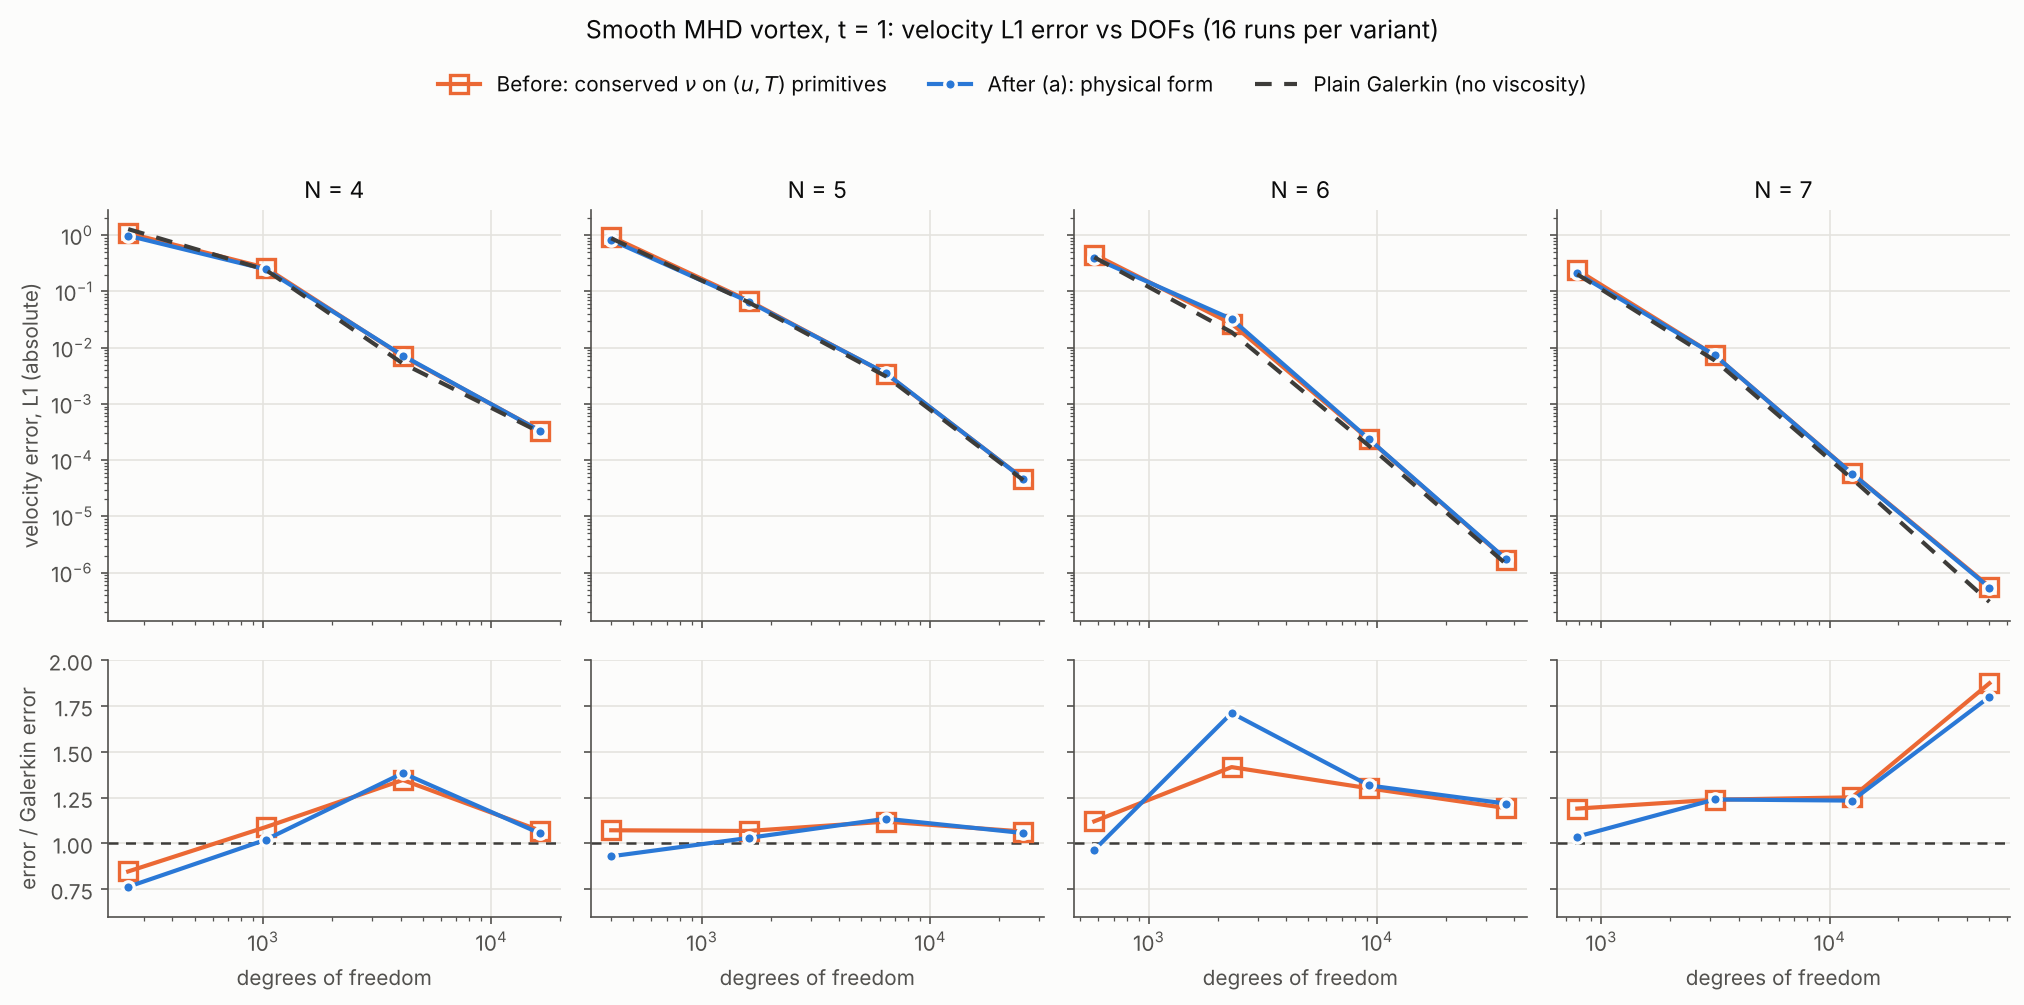
\includegraphics[width=\textwidth]{smoothVortex_test.png}
\end{center}
{\footnotesize\setlength{\tabcolsep}{3.2pt}
\begin{longtable}{@{}rrr*{3}{r}*{3}{r}*{3}{r}@{}}
\toprule
$N$ & mesh & DOFs & \multicolumn{3}{c}{velocity $L^1$ error} & after & before & after & \multicolumn{3}{c}{observed order}\\
\cmidrule(lr){4-6}\cmidrule(lr){10-12}
 & & & before & after (a) & Galerkin & /before & /Gal. & /Gal. & before & after & Gal.\\
\midrule\endhead
\bottomrule\endfoot
4 & $4^2$ & 256 & $1.09\times10^{0}$ & $9.82\times10^{-1}$ & $1.29\times10^{0}$ & 0.901 & 0.85 & 0.76 &  &  & \\
4 & $8^2$ & 1024 & $2.65\times10^{-1}$ & $2.48\times10^{-1}$ & $2.44\times10^{-1}$ & 0.936 & 1.09 & 1.02 & 2.04 & 1.98 & 2.40\\
4 & $16^2$ & 4096 & $7.05\times10^{-3}$ & $7.25\times10^{-3}$ & $5.24\times10^{-3}$ & 1.028 & 1.35 & 1.38 & 5.23 & 5.10 & 5.54\\
4 & $32^2$ & 16384 & $3.33\times10^{-4}$ & $3.28\times10^{-4}$ & $3.11\times10^{-4}$ & 0.986 & 1.07 & 1.05 & 4.40 & 4.46 & 4.07\\\midrule
5 & $4^2$ & 400 & $9.45\times10^{-1}$ & $8.20\times10^{-1}$ & $8.82\times10^{-1}$ & 0.867 & 1.07 & 0.93 &  &  & \\
5 & $8^2$ & 1600 & $6.86\times10^{-2}$ & $6.61\times10^{-2}$ & $6.42\times10^{-2}$ & 0.964 & 1.07 & 1.03 & 3.78 & 3.63 & 3.78\\
5 & $16^2$ & 6400 & $3.46\times10^{-3}$ & $3.51\times10^{-3}$ & $3.09\times10^{-3}$ & 1.014 & 1.12 & 1.14 & 4.31 & 4.24 & 4.38\\
5 & $32^2$ & 25600 & $4.70\times10^{-5}$ & $4.66\times10^{-5}$ & $4.41\times10^{-5}$ & 0.992 & 1.07 & 1.06 & 6.20 & 6.23 & 6.13\\\midrule
6 & $4^2$ & 576 & $4.55\times10^{-1}$ & $3.91\times10^{-1}$ & $4.06\times10^{-1}$ & 0.861 & 1.12 & 0.96 &  &  & \\
6 & $8^2$ & 2304 & $2.67\times10^{-2}$ & $3.23\times10^{-2}$ & $1.89\times10^{-2}$ & 1.209 & 1.42 & 1.71 & 4.09 & 3.60 & 4.43\\
6 & $16^2$ & 9216 & $2.34\times10^{-4}$ & $2.37\times10^{-4}$ & $1.80\times10^{-4}$ & 1.012 & 1.30 & 1.32 & 6.84 & 7.09 & 6.72\\
6 & $32^2$ & 36864 & $1.68\times10^{-6}$ & $1.72\times10^{-6}$ & $1.41\times10^{-6}$ & 1.020 & 1.19 & 1.22 & 7.12 & 7.11 & 6.99\\\midrule
7 & $4^2$ & 784 & $2.40\times10^{-1}$ & $2.10\times10^{-1}$ & $2.02\times10^{-1}$ & 0.872 & 1.19 & 1.04 &  &  & \\
7 & $8^2$ & 3136 & $7.36\times10^{-3}$ & $7.37\times10^{-3}$ & $5.94\times10^{-3}$ & 1.001 & 1.24 & 1.24 & 5.03 & 4.83 & 5.09\\
7 & $16^2$ & 12544 & $5.85\times10^{-5}$ & $5.77\times10^{-5}$ & $4.68\times10^{-5}$ & 0.986 & 1.25 & 1.23 & 6.97 & 7.00 & 6.99\\
7 & $32^2$ & 50176 & $5.66\times10^{-7}$ & $5.43\times10^{-7}$ & $3.02\times10^{-7}$ & 0.960 & 1.87 & 1.80 & 6.69 & 6.73 & 7.28\\
\end{longtable}}
\noindent\textbf{Reading.} On the two finest meshes the two operators are within $-4\%$ and $+3\%$ of each other in $L^1$
and their observed orders agree to $\pm0.25$ (finest pair: 4.40/4.46, 6.20/6.23, 7.12/7.11, 6.69/6.73 for $N=4,\dots,7$);
on the coarsest ($4^2$) the physical form is 10--14\% lower in $L^1$ and 7--28\% lower in $L^\infty$; the one point
where it is clearly worse is $N=6$ on $8^2$ ($1.21\times$ in $L^1$). Both stay within a factor of 1.05--1.4 of the
plain Galerkin error at $N\le6$ on the finest meshes, and both are $\approx1.8$--$1.9\times$ Galerkin at $N=7$ on $32^2$,
where the viscosity itself, common to both, sets the gap. The change of operator therefore does not alter the
accuracy picture of this case; it makes the operator the one the case documents.

\section{Positivity}
\begin{itemize}[leftmargin=*]
\item \mj{\code{:lpositivity} false}; \mj{no stage limiter}; \mj{no state modification of any kind}.
\item No flux-only floor either: \code{pressure\_mhd} is the unguarded Orszag--Tang one.
\item None is needed by design: the data are smooth, $\min p = 1-1/(8\pi^2)\approx0.987$ initially (at $r=1$), and
the case measures accuracy, not robustness.
\end{itemize}

\section{Observations: code versus comments}
\begin{enumerate}[leftmargin=*]
\item Since \code{f9cdb02} the deck, \code{user\_primitives.jl} and the kernel agree (the physical form above).
\item Everything else in the deck matches its comments (domain norms, hold 2, no floor, no cutoff,
the residual sensor).
\item \textbf{[Changed in \code{b956ccd}.]} The deck no longer sets \code{:dsgs\_freeze\_stage} unless
\code{JEXPRESSO\_SV\_FREEZE} is given, so the \code{DSGS\_MHD} default applies: the coefficient frozen per step. The
before-and-after test above (\emph{Test: before against after}) was run per stage.
\item \textbf{[Changed in \code{22c0907}.]} The deck runs the smoothness cutoff $c=10^{-3}$ by default, as the Alfv\'en wave
does (\code{dsgsCutoff.pdf}): without it the residual sensor reads the $O(\Delta t^2)$ truncation error of its own time
difference on the moving vortex and caps \dsgs{} near order 4 from $N=5$ on. Its records \code{dsgs} are now the runs with
the cutoff; \code{JEXPRESSO\_SV\_CUTOFF=0} runs without it (\code{dsgs\_nocut}).
\end{enumerate}

% Shared appendix: where each mechanism lives in the source (branch sm/MHD, commit dcc3653).
\section*{Appendix: code map (branch \branch, commit \commit)}
\addcontentsline{toc}{section}{Appendix: code map}
{\small
\begin{longtable}{@{}L{0.47\textwidth}L{0.47\textwidth}@{}}
\toprule
\textbf{Mechanism} & \textbf{Where (file:line)}\\
\midrule\endhead
\bottomrule\endfoot
Deck defaults of every \code{:dsgs\_*} key & \code{src/io/mod\_inputs.jl:1085--1376}\\
Deck defaults of \code{:lpositivity}, floors, report & \code{src/io/mod\_inputs.jl:456--477}\\
\code{:positivity\_method}; rebuild of the RK solver & \code{src/io/mod\_inputs.jl:828--838}\\
\dsgs{} history rotation, stage weights, hold, freeze & \code{src/kernel/operators/rhs.jl:927--984}\\
Stencil selection \code{\_dsgs\_stencil} & \code{rhs.jl:141}\\
Hold length \code{\_dsgs\_hold\_steps} ($\max(2,H)+1$ rotations) & \code{rhs.jl:182}\\
Residual right-hand side (element / legacy / Dirichlet) & \code{rhs.jl:188--280}; legacy fill \code{rhs.jl:282}; boundary zeroing \code{rhs.jl:313, 346}\\
1D \code{DSGS\_MHD} dispatch & \code{rhs.jl:1398--1470}\\
2D \code{DSGS\_MHD} dispatch (sets \code{dsgs\_ref\_weight}, \code{dsgs\_split\_energy}, \code{dsgs\_nodal\_rho}) & \code{rhs.jl:1517--1610}\\
2D viscous assembly \code{\_viscous\_rhs\_el\_2d\_dsgs!} & \code{rhs.jl:1796}\\
2D weak viscous flux \code{\_expansion\_visc!} (conserved flag, ref.\ weight, split energy, $\tau\cdot\bv$, resistive work) & \code{rhs.jl:2943--3210} (\code{lcons} 2959, weight 2978, split 3050, $\tau\cdot\bv$ 3076, $\eta\,\bB\cdot\nabla\bB$ 3091)\\
1D weak viscous flux & \code{rhs.jl:2823}; element loop \code{rhs.jl:1321}\\
2D \code{DSGS\_MHD} element kernel & \code{src/kernel/physics/SGS.jl:1598--1912}\\
1D \code{DSGS\_MHD} element kernel & \code{SGS.jl:1929--2120}\\
Nodal kernels (off in every MHD deck; BW can switch it on with \code{JEXPRESSO\_BW\_NODAL=1}) & \code{SGS.jl:2144} (1D), \code{SGS.jl:2515} (2D)\\
Normalization floor \code{\_dsgs\_denom}, \code{:dsgs\_rel} multiplier & \code{SGS.jl:676--679}; set per call in \code{rhs.jl:192}\\
Smoothness cutoff \code{\_dsgs\_cut} & \code{SGS.jl:703}\\
\code{SGS\_diffusion(::DSGS\_MHD)} (nodal-$\rho$ switch) & \code{SGS.jl:547--569}\\
Element length $\Delta^{elem}_K$ (2D: min of corner extents) & \code{src/kernel/mesh/mesh.jl:6430--6457}; 1D $\Delta x$: \code{mesh.jl:5863}\\
\code{uprimitive} width ($n_{eqs}+2$ in 2D, $n_{eqs}+1$ in 1D) & \code{src/kernel/globalStructs.jl:139--153}\\
Realizability repair (\code{"repair"}, unused by the MHD decks) & \code{src/kernel/positivity/Positivity.jl:294}; driver \code{positivity\_driver.jl:124}; called in \code{rhs.jl:821}\\
Conservative element limiter (\code{"conservative"}) & \code{Positivity.jl:433--559}; driver \code{positivity\_driver.jl:245--337}\\
Main \code{solve} call (\code{saveat} non-empty $\Rightarrow$ \code{calck = true}) & \code{src/kernel/solvers/TimeIntegrators.jl:855}\\
\end{longtable}}
\noindent\small Stage-limiter calls in \code{CarpenterKennedy2N54}: with \code{williamson\_condition = false}
the limiter is called before the right-hand side of stages 2--5 and once after stage 5
(OrdinaryDiffEq v6.90/v6.95, \code{low\_storage\_rk\_perform\_step.jl}). In OrdinaryDiffEq
\code{calck = true} forces \code{williamson\_condition = false} in the 2N cache, and Jexpresso's
\code{solve} passes a non-empty \code{saveat}, so this holds for every deck that hands the solver
a stage limiter. (Jexpresso ships no \code{Manifest.toml}; the package version is whatever the
environment resolves, and the check above was made against v6.90/v6.95.)

\end{document}
